\chapter{BÀI TOÁN LỌC RÁC TIN TỨC VÀ CÁC PHƯƠNG PHÁP TIẾP CẬN PHỔ BIẾN}
\ifpdf
    \graphicspath{{Chapter2/Chapter2Figs/PNG/}{Chapter2/Chapter2Figs/PDF/}{Chapter2/Chapter2Figs/}}
\else
    \graphicspath{{Chapter2/Chapter2Figs/EPS/}{Chapter2/Chapter2Figs/}}
\fi

\section{Mở đầu}
Chương này sẽ giới thiệu bài toán lọc rác tin tức cho hệ thống phát hiện tin nóng. Trình bày cơ sở lý thuyết và phát biểu bài toán lọc rác tin tức. Cuối cùng trình bày một số phương pháp tiếp cận bài toán lọc rác tin tức  và các kiến thức liên quan.
\section{Giới thiệu bài toán} %Topic Detection and Tracking}
	\subsection{Các khái niệm cơ bản}
  Để có thể xác định khái niệm rác, ta phải hiểu được khái nhiệm "tin nóng". Le \cite{An:2017} đã định nghĩa khái niệm "tin nóng" như sau:
	\begin{itemize}
    \item \textit{Tin nóng (Hot news)}: những tin viết về một sự kiện mới xảy ra, có tính thời sự, có tầm ảnh hưởng rộng, thu hút được sự chú ý, quan tâm của cộng đồng.
	\end{itemize}

  Ngoài ra Gy ̈ongyi và Garcia-Molina định nghĩa "đăng rác" như sau: 
	\begin{itemize}
    \item \textit{Đăng rác (Spamming)}: các hành động có chủ đích của con người nhầm thiên vị tính liên quan của một trang web nào đó, làm sai lệch giá trị của trang web.
	\end{itemize}

  Từ các khái niệm trên ta có định nghĩa "rác" cho bài toán như sau:

  \textbf{Định nghĩa:} Rác là các tin không mang tính chất sự kiện, thời sự, và làm sai lệch kết quả phân tích và xử lý dữ liệu của hệ thống phân loại tin tức. 

  Từ định nghĩa trên ta có thể xác định được các loại tin sẽ được xem là rác:
  \begin{itemize}
    \item \textit{Quảng cáo}: các bài quảng cáo, giới thiệu sản phẩm, các chương trình khuyển mãi, trúng thưởng.
    \item \textit{Tuyển dụng}: các bài đăng tuyển dụng, giới thiệu việc làm của các tổ chức, doanh nghiệp.
    \item \textit{Chia sẻ}: các bài chia sẻ mẹo vặt, thủ thuật, tâm sự, chuyện đời tư, giới thiệu ẩm thực, thời trang, hoặc các kiến thức chung.
  \end{itemize}

	\subsection{Bài toán phân lớp văn bản}
  Bài toán phân lớp văn bản là bài toán có lịch sử lâu đời, một số ghi nhận cho thấy nó bắt đầu từ những năm 1800s, tuy nhiên tới nay vẫn chưa có một sự thống nhất nào về phương pháp tốt nhất cho bài toán phân lớp \cite{zechner:history}. 
  
	Theo Zechner \cite{zechner:history}, bài toán phân lớp văn bản gồm các thành phần chính cần quan tâm: 
		\begin{itemize}
			\item Loại phân lớp: supervised hoặc unsupervised.
			\item Mục tiêu: đối tượng thành phần của văn bản mà ta muốn quan tâm.
			\item Kho từ vựng: kích thước và chất lượng của kho từ vựng ảnh hưởng lớn đến việc phân lớp.
			\item Features: đặc trưng của văn bản dùng cho việc phân lớp.
			\item Bộ phân lớp: thuật toán máy học dùng cho việc phân lớp.
		\end{itemize}

	\subsection{Bài toán lọc rác tin tức}
  Bài toán lọc rác hay còn được biết đến như là bài toán phát hiện rác (Spam detection) là một dạng bài toán phân lớp văn bản nhị phân. Tức là chỉ có hai lớp: "rác" và "không rác". Đối với hệ thống phát hiện tin nóng cũng như các hệ thống phân tích và xữ lý dữ liệu khác, việc phát hiện và lọc rác phải được diễn ra trước khi quá trình phân tích và xử lý dữ liệu bắt đầu để đảm bảo quá trình phân tích và xử lý dữ liệu chính xác và đáng tin cậy.

  Mặc dù nguồn dữ liệu mà chúng ta quan tâm là tin tức từ các trang báo điện tử chính thống, số lượng nguồn tin, chủ đề tin và số lượng tin rất lớn dẫn đến việc chất lượng dữ liệu tin tức không được đảm bảo cũng như tính chất dữ liệu không được phù hợp với nhu cầu của hệ thống. Do đó việc lọc rác tin tức là cần thiết cho việc khai thác và sử dụng nguồn dữ liệu tin tức một các hiệu quả.

  \subsection{Phát biếu bài toán lọc rác tin tức cho hệ thống phát hiện tin nóng}
  Cho trước một bài báo $d_i$i. Mục tiêu của bài toán là tìm ra được nhãn $l_i$ của bài báo $d_i$ và nhãn đó nhận một trong hai giá trị: "rác" và "không rác".
	
\section{Các nghiên cứu liên quan}
Vấn đề phát hiện và lọc rác là một vấn đề lâu đời và kinh điển đối với bài toán phân lớp văn bản. Do đó số lượng nghiên cứu xoay quan vấn đề này cũng rất lớn và đa dạng. Phần lớn các nghiên cứu cho đến ngày nay tập trung vào việc phát hiện rác cho email và web. 

Sahami và cộng sự \cite{Sahami1998ABA} sử dụng các tiếp cận Bayesian vào vấn đề lọc rác cho email. Thực nghiệm cho thấy các bộ phân lớp đạt được hiệu suất cao hơn khi ta cân nhắc các tính năng đặc trưng theo domain và nội dung văn bản của email. Ngày nay thì các phương pháp phát hiện và lọc rác cho email đã khá hoàn thiện, và các phương pháp phát hiện và lọc rác Bayesian được áp dụng rộng rãi trong các email client và server.

Vấn đề phát hiện rác cho web thì khó khăn hơn vì độ lớn và tốc độ thay đổi nhanh chóng. Gy\"{o}ngyi và cộng sự \cite{Gyongyi:2004:CWS:1316689.1316740} đề xuất sử dụng thuật toán TrustRank để đo kiểm điểm tin cậy của đồ thị Web. Dựa trên điểm tin cậy, các trang web tốt sẽ được đánh giá cao hơn va những trang web xấu có thể được search engine bỏ qua. 

\section{Giới thiệu một số phương phát trừu tượng hóa dữ liệu văn bản} \label{distances}
Do máy tính không thể đọc hiểu và xử lý được dữ liệu thuần văn bản, ta cần có một phương pháp trừu tượng hóa dữ liệu văn bản thành các con số mà máy tính có thể hiểu được.
\subsection*{Term Frequency - Inverse Document Frequency (TF-IDF)}
Trong lĩnh vực thu thập thông tin, TF-IDF là một dữ liệu số dùng để thể hiện độ quan trọng của một từ trong một một tập hợp hoạc một kho từ vựng \cite{rajaraman_ullman_2011}. Nó thường được dùng trong việc thu thập thông tin, text mining và user modeling. Giá trị của TF-IDF tăng theo tỉ lệ với số lần một từ xuất hiện trong một văn bản, nhưng thường bị giảm lại theo tần xuất của từ đó trong toàn kho từ vựng, vì một từ có thể chỉ đơn giản là nó phổ biến hơn các từ khác. Ngày nay, TF-IDF là một trong những phương pháp tính trọng số cho các từ phổ biến nhất; 83\% các hệ thống khuyến nghị dựa trên văn bản trong lĩnh vực thư viện điện tử sử dụng TF-IDF \cite{Beel2016}.

TF-IDF gồm có hai thành phần chính Term Frequency (TF) và Inverse Document Frequency (IDF).

TF của từ $t$ trong văn bản $d$ được thể hiện dưới dạng $tf(t,d)$. Ta có nhiều cách tính TF, trong đó cách đơn giản nhất là đếm số lần một từ xuất hiện trong một văn bản. Nếu ta gọi số lần từ $t$ xuất hiện trong văn bản $d$ là $f_{t,d}$ thì ta có $tf(t,d) = f_{t,d}$

IDF là thước đo lượng thông tin một từ cung cấp, có nghĩa là liệu từ đó hiếm gặp hay xuất hiện xuyên suốt trong kho từ vựng. IDF được tính bằng công thức:
\begin{equation}
  idf(t, D) = \log\frac{N}{1 + \abs{\{d \in D: t \in d\}}}
\end{equation}

Trong đó:
\begin{itemize}
  \item $D$: kho từ vựng.
  \item $N$: số lượng văn bản trong kho từ vựng.
  \item $\abs{\{d \in D: t \in d \}}$: số lượng văn bản và có xuất hiện từ $t$. 
\end{itemize}
	\subsection*{Word Vector}
  Word vector là một hình thức biểu diễn các từ trong một kho từ vựng dưới dạng các vector. Các từ thường xuất hiện cùng nhau trong các nhiều ngữ cảnh khác nhau thì sẽ được biểu diễn bằng các vector gần với nhau trong không gian vector \cite{mikolov:word2vec}. Tập hợp các kỹ thuật để nhận vào input là một kho từ vựng và cho ra một không gian vector tương ứng được gọi là word2vec.

  Word vector thường được sử dụng trong các công cụ tìm kiếm và dịch thuật do nó cung cấp thông tin về sự tương qua ngữ nghĩa giữa các từ và các ngữ cảnh cũng như giữa các từ với nhau.

\section{Các phương pháp tiếp cận phổ biến}
Phân lớp là quá trình xác định xem một đối tượng sẽ thuộc về lớp nào dựa trên việc quan sát các đối tượng khác mà lớp của chúng đã được xác định từ trước. Thông thường, các đối tượng cần phân lớp sẽ được phân tích thành các thuộc tính có thể đo đếm được. Một thuật toán dùng để phân lớp, hay còn được gọi là một bộ phân lớp, sẽ dựa trên các thuộc tính đó để ánh xạ các đối tượng input mới vào lớp của chúng. Đây là một trong những tác vụ chính của lĩnh vực khai thác dữ liệu.

Bài toán phân lớp bao gồm nhiều thuật toán khác nhau, trong phạm vi của khóa luận chúng ta sẽ chỉ quan tâm đến các thuật toán: Support vector machine, Naive Bayes, và J48 decision tree.
\subsection{Thuật toán phân lớp Support Vector Machine (SVM)}
\subsubsection{Ý tưởng}
Support vector machine hay còn gọi là support vector network là một thuật toán phân lớp dành cho các bài toán phân lớp nhịphân. SVM thực hiện phân lớp bằng việc ánh xạ các vector lên một không gian nhiều chiều. Trên không gian này sẽ sinh ra một mặt phẳng quyết định tuyến tính phân tách hai lớp dữ liệu \cite{Cortes1995}.
	\subsubsection{Minh họa thuật toán}
		Giả sử ta có dữ liệu như hình vẽ. Đường tròn thể hiện ngưỡng khoảng cách để một document được xem là first story hay không, chọn ngưỡng giá trị 0.8. Ta có sẵn 4 document và 1 document mới vào hệ thống như sau:
		\begin{center}
					doc1 = (3,4,1,2)\\
				doc2 = (1,1,5,6)\\
				doc3 = (1,2,4,4)\\
				doc4 = (3,5,1,1)\\
				newDoc = (2,1,4,5)\\
		\end{center}
		\begin{table}[H]
			\centering
			\begin{tabular}{|p{1.5cm}|p{1.5cm}|p{1.5cm}|p{1.5cm}|p{1.5cm}|p{1.5cm}|}
				\hline
				& doc1 & doc2 & doc3 & doc4 & \textbf{newDoc} \\
				\hline 
				doc1 & 1 & 0.55202 & 0.6903 	& 0.973729 & 0.646058 \\
				doc2 &   & 1 		& 0.973479 	& 0.398962 & 0.984525 \\
				doc3 &   &   		& 1			& 0.575396 & 0.969572 \\
				doc4 &   &  		&  			& 1 	& 0.491473 \\
				newDoc &   &  		&  			&   	& 1 \\
				\hline
			\end{tabular}
			\caption{Độ tương đồng cosine giữa các document} \label{tab:table_1_1}
		
		\end{table}
		Ta có thể thấy document tương tự nhất của newDoc là doc2 (0.984525), lớn hơn ngưỡng cho trước (0.8), do đó newDoc được cho vào chung cụm với doc2 và không phải là một first story.
	
		\begin{figure}[H]
			\begin{center}
				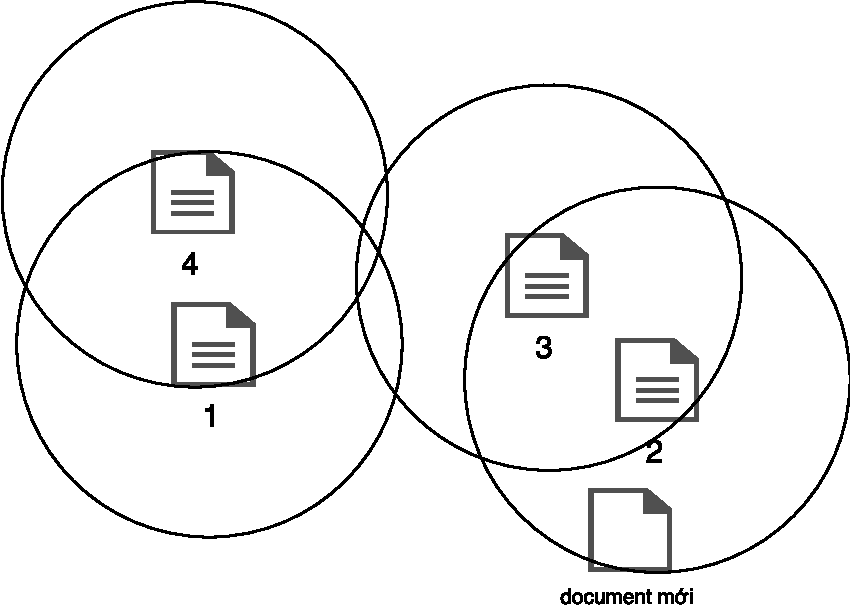
\includegraphics[width=0.9\linewidth]{NNS.pdf}
				\caption{Cách xử lý một document mới trong thuật toán Nearest Neighbor Search}
			\end{center}
		\end{figure}
		
	\subsubsection{Mã giả}
		\begin{algorithm}[H]
			\caption{Phát hiện tin nóng dựa trên k-Nearest neighbor}
			\begin{algorithmic}[1]
				\REQUIRE luồng bài viết từ Twitter, giá trị ngưỡng MergeThreshold
				\ENSURE các cụm bài viết
				\ForEach{document $d$ trong toàn bộ dữ liệu}
					\State $S(d) \leftarrow \emptyset$
					\ForEach{term $t$ trong document $d$}
						\ForEach{document $d'$ trong $index[t]$}
							\State cập nhật độ tương đồng $similarity(d,d')$
							\State $S(d) \leftarrow S(d) \cup d'$
						\ENDFOR 
						\State $index[t] \leftarrow index[t] \cup d$ (thêm document $d$ vào index của term t)
					\ENDFOR
					\STATE similarity score của d: $similarity_{max}(d) \leftarrow 0$
					
					\ForEach{document $d'$ trong S(d)}
						\IF{$similarity(d,d') > similarity_{max}(d)$}
							\STATE $similarity_{max}(d) \leftarrow similarity(d,d')$
						\ENDIF
					\ENDFOR
					\IF{$similarity_{max}(d) < MergeTheshold$}
						\STATE d là một first story
					\ELSE
					
					\ENDIF
				\ENDFOR	
				
			\end{algorithmic}
		\end{algorithm}
		Chú thích thuật toán:
		\begin{itemize}
			\item $MergeThreshold$: ngưỡng để xét một document có phải là first story hay không
			\item $S(d)$: tập document có ít nhất 1 term chung với $d$
			\item $similarity(d,d')$: độ tương đồng giữa document $d$ và $d'$, có thể sử dụng các độ đo ở mục~\ref{distances}
			\item $index(t)$: danh sách cách document có chứa term $t$
			\item $dis_{min}(d)$: khoảng cách giữa document $d$ với document gần nhất
		\end{itemize}
		
	\subsubsection{Ưu điểm, hạn chế}
		Ưu điểm:
		\begin{itemize}
			\item Đơn giản và dễ cài đặt.
			\item Có thể chọn nhiều độ đo khoảng cách khác nhau.
			\item Thích nghi tốt với nhiều loại dữ liệu.
		\end{itemize}
		Nhược điểm:
		\begin{itemize}
			\item Chi phí tính toán cao do phải lưu trữ và tính toán trên toàn bộ dữ liệu, không thể áp dụng cho luồng dữ liệu không liên tục.
			\item Độ chính xác giảm khi số chiều của dữ liệu tăng cao.
		\end{itemize}
%========================================================================================================================
	
\subsection{Thuật toán gom cụm có Boost trọng số cho Named Entity}
	\subsubsection{Ý tưởng}
	Cách tiếp cận được đề xuất bởi Phuvipadawat là gom cụm các bài viết theo độ tương tự nội dung, với điểm nhấn là tăng giá trị tương đồng của các bài viết nếu chúng cùng đề cập đến một thực thể có tên (Named entity) nào đó \cite{SwitPhuvipadawat}. Mỗi cụm thu được sẽ ứng với một sự kiện phát hiện được, với document cũ nhất làm đại diện cho cụm đó.
	
	Theo Phuvipadawat, một đặc điểm của các bài viết trên Twitter là thường có nội dung khá ngắn (tối đa 140 kí tự, và ngắn hơn nữa sau khi tiền xử lý loại bỏ stop words). Việc sử dụng phương pháp TF-IDF truyền thống để tính độ tương đồng có thể không đạt được kết quả tốt do không có nhiều term để tìm ra sự tương đồng giữa các document. Vì thế tác giả đã đưa ra phương pháp tăng trọng số cho các danh từ riêng (Named Entity), qua đó tăng độ tương đồng giữa những bài viết cùng thảo luận về một sự vật, sự việc cụ thể nào đó.
		
	Khi một document $d$ mới được đưa vào hệ thống, ta so sánh độ tương đồng giữa $d$ với tất cả cụm hiện có thông qua document đầu tiên trong cụm. Ta chọn ra cụm có độ tương đồng với $d$ cao nhất, gán $d$ vào cụm đó nếu độ tương đồng vượt ngưỡng định trước, ngược lại ta tạo cụm mới với $d$ là document đầu tiên của cụm.
	
	\subsubsection{Minh họa thuật toán}
	Giả sử ta có một số document đã được gom nhóm sẵn thành 3 cụm như hình, ngưỡng MergeThreshold = 0.7, mỗi cụm có một firstDoc làm đại diện. Đường tròn thể hiện ngưỡng khoảng cách để một document được xem là first story hay không.\\
	
	Khi một document mới (newDoc) vào hệ thống: 
	\begin{itemize}
		\item Bước 1: So sánh newDoc với từng firstDoc của từng cụm:\\ 
		$similarity(newDoc, g1.firstDoc) = 0.6$\\
		$similarity(newDoc, g2.firstDoc) = 0.5$\\
		$similarity(newDoc, g3.firstDoc) = 0.35$%Tính ra độ tương đồng
		\item Bước 2: Tìm cụm có firstDoc tương tự với newDoc nhất: Chọn được cụm $g1$%chọn rõ g1...
		\item Bước 3: $similarity(newDoc, g1.firstDoc) = 0.6$ nhỏ hơn MergeThreshold: Tạo cụm g4 với $g4.firstDoc = newDoc$.
	\end{itemize}
	
	%Cho số cụ thể?? 
	\begin{figure}[ht]
		\begin{center}
			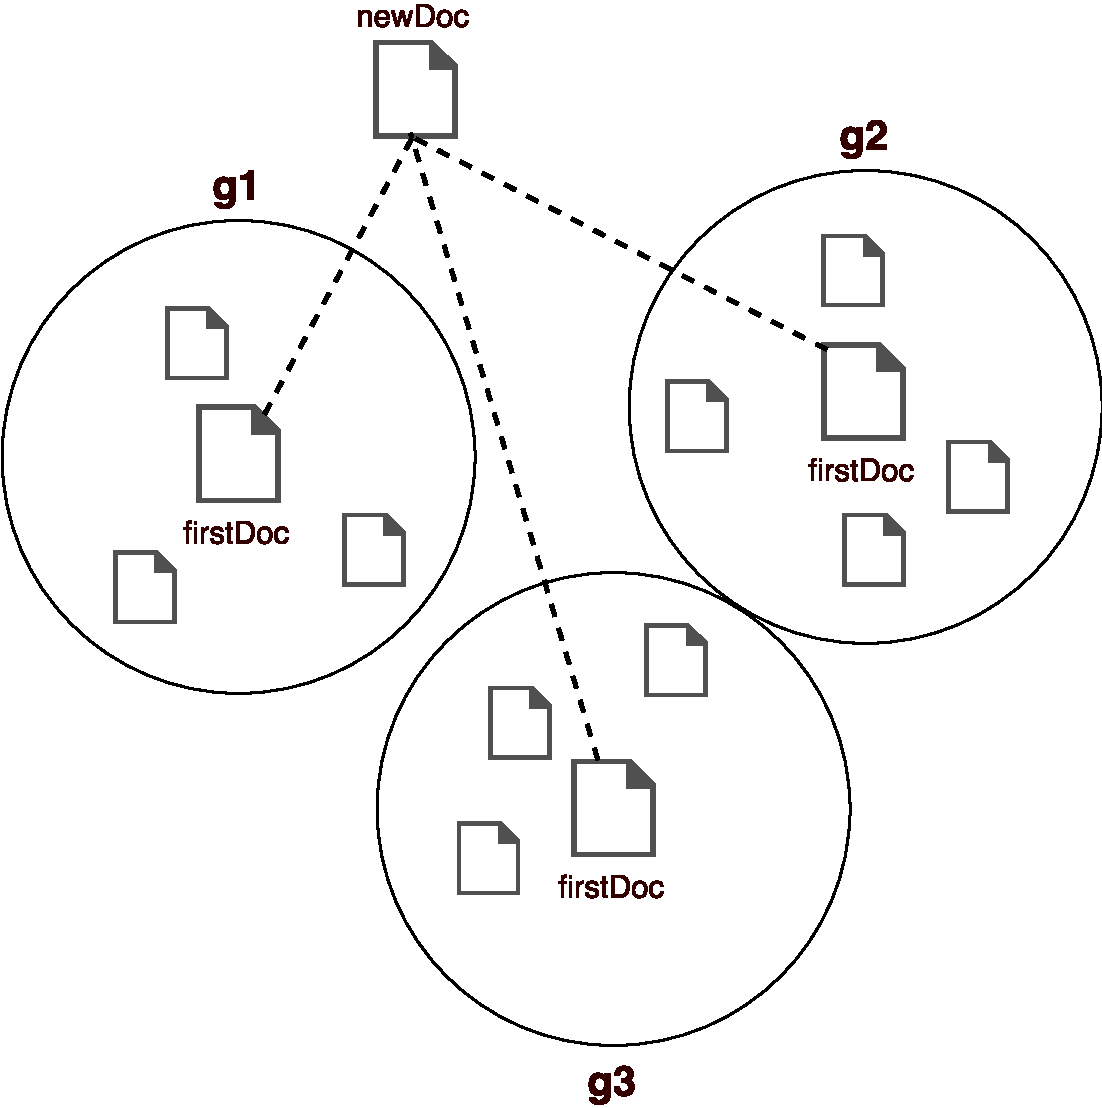
\includegraphics[width=0.65\textwidth]{Clustering_NER2.pdf}
			\caption{Cách xử lý một document mới theo thuật toán Boost Named Entity}
		\end{center}
	\end{figure}
	
	\subsubsection{Mã giả}
	\begin{algorithm}[H]
		\caption{Phát hiện tin nóng sử dụng gom cụm theo nội dung, boost Named Entity}
		\begin{algorithmic}[1]
			\REQUIRE luồng bài viết từ Twitter, giá trị ngưỡng MergeThreshold
			\ENSURE các cụm bài viết ứng với mỗi story phát hiện được, có thứ tự xếp hạng giữa các cụm

			\ForEach{document $d$ trong toàn bộ dữ liệu}
				\State $MaxScore_d \leftarrow 0$
				\State $IDMaxScore_d \leftarrow \emptyset$
				\ForEach{cụm g trong tập hợp cụm G}
%					\State tính $Score_d[g]$: độ tương đồng giữa $d$ với $g.firstDoc$, chỉ dùng một số topTerms của $g$
					\State tính $Score_d[g] \leftarrow similarity(d, g.firstDoc)$
					
					\IF{$MaxScore_d < Score_d[g]$}
						\State $MaxScore_d \leftarrow Score_d[g]$
						\State $IDMaxScore_d \leftarrow g.groupID$
					\ENDIF
				\ENDFOR
				
				\IF{$MaxScore_d$ > MergeThreshold}
					\State gán $d$ vào cụm $IDMaxScore_d$
				\ELSE
					\State tạo cụm $g_{new}$
					\State $g_{new}.firstDoc \leftarrow d$
				\ENDIF
			\ENDFOR
		\end{algorithmic}
	\end{algorithm}
	Chú thích thuật toán:
	\begin{itemize}
		\item $MaxScore_d$: chứa độ tương đồng lớn nhất giữa document d và các cụm đã có
		\item $IDMaxScore_d$: ID của cụm tương đồng nhất với document d
		\item $Score_d[g]$: độ tương đồng giữa document d với cụm g 
		\item $MergeThreshold$: ngưỡng để xét một document có thuộc về cụm/có là first story hay không
	\end{itemize}
	Độ tương đồng giữa 2 document được tính bằng các công thức sau:
	\begin{equation}
			similarity(d_1, d_2) = \sum_{t \in d_1,\ t \in g.topTerms}[tf(t, d_2) \times idf(t) \times boost(t)]
	\end{equation}
	\begin{equation}
		tf(t, d) = \frac{count(t \in d)}{size(d)}
	\end{equation}
	\begin{equation}
		idf(t) = 1 + \log\frac{N}{count(m\ has\ t)}
	\end{equation}
	Các kí hiệu: 
	\begin{itemize}
		\item $similarity(d_1, d_2)$: độ tương đồng giữa document $d_1$ và document $d_2$
		\item $boost(t)$: giá trị boost cho term t, nếu t là một danh từ riêng (Named Entity) thì boost(t) > 1, ngược lại boost(t) = 1
		\item $tf(t, d)$: tần suất xuất hiện (theo phần trăm) của term t trong document d
		\item $count(t \in d)$: tần suất term t xuất hiện trong trong document d
		\item $size(d)$: số lượng term của document d
		\item $idf(t)$: giá trị inverse document frequency của term t
		\item $N$: tổng số document trong hệ thống
		\item $count(m\ has\ t)$: số document có chứa term t
	\end{itemize}

	\subsubsection{Ưu điểm, hạn chế}
	Ưu điểm:
	\begin{itemize}
		\item Dễ gom nhóm được các sự kiện bàn về cùng thực thể nào đó.
	\end{itemize}
	Nhược điểm:
	\begin{itemize}
		\item Chất lượng kết quả gom cụm phụ thuộc một phần vào việc phát hiện được thực thể có tên.
	\end{itemize}

%========================================================================================================================
\subsection{Thuật toán Locality Sensitive Hashing}
	\subsubsection{Ý tưởng}
%	(O(nd) với n là số lượng document hiện có và d là số chiều của mỗi document)
	Thuật toán tìm kiếm láng giềng gần nhất tốn rất nhiều chi phí khi lượng dữ càng lớn. Thay vào đó, ta có thể giải bài toán tìm \textit{xấp xỉ} láng giềng gần nhất. Một thuật toán để giải quyết bài toán này là \textit{Locality Sensitive Hashing (LSH)} được đề xuất bởi Piotr Indyk và cộng sự \cite{Indyk:LSH-Definition}.
	
	LSH hoạt động bằng cách chia không gian biểu diễn dữ liệu thành nhiều vùng riêng biệt bằng một tập các siêu phẳng ngẫu nhiên. Ta có thể xem mỗi cách chia không gian này ứng với một hash table, và số bit của hash code bằng với số lượng siêu phẳng đã dùng để chia không gian. Mỗi khi một document mới vào hệ thống, ta tính hash code của nó. Khi cần tìm láng giềng cho một document, ta chỉ cần so sánh nó với các document thuộc chung vùng không gian (ứng với một bucket trong hash table), nhờ đó giảm đáng kể chi phí tính toán.
	
%	Ta có thể thấy khi tăng số lượng siêu phẳng lên thì số lượng document rơi vào cùng một vùng không gian sẽ càng giảm, do kích cỡ của vùng không gian nhỏ, th
	
	Vì các siêu phẳng được chọn một cách ngẫu nhiên, nên đôi khi các document dù gần nhau vẫn có thể bị phân vào vùng khác nhau. Do đó ta thường dùng cùng lúc nhiều hash table để tăng thêm khả năng tìm được láng giềng gần nhất.	
%	LSH sử dụng một họ hash function (hàm băm) có đặc điểm: những documents càng tương đồng với nhau thì càng có khả năng trùng hash code (mã băm) với nhau. Mỗi document mới sẽ được đưa qua hash function tính toán, và sau đó được so sánh với các document có cùng hash code với nó.\\

	\subsubsection{Minh họa cách tính hash code cho LSH}
%	Xét trường hợp một document $d$ biểu diễn dưới dạng vector $d = (0,1,0,1,1,1,0)$, và ta chọn sử dụng hash code có 4 bit (dùng 4 siêu phẳng để chia không gian dữ liệu).\\
%	Mỗi hash table được khởi tạo bằng cách: tạo 4 vector ngẫu nhiên ứng với 4 siêu phẳng, số chiều bằng với số chiều vector $d$
%	Cách tính hash code của document $d$ trong một hash table như sau: lần lượt tính tích vô hướng của vector $d$ với từng vector của siêu phẳng, nếu tích dương thì bit đó có giá trị 1, nếu tích âm thì có giá trị 0. 
		
	Giả sử ta có không gian biểu diễn document gồm 7 từ/term khác nhau (8 chiều). Xét một document $d$ biểu diễn dưới dạng vector $d = (0,1,0,1,1,1,0)$, và ta chọn sử dụng hash code có 4 bit (dùng 4 siêu phẳng để chia không gian dữ liệu).
	
	Mỗi hash table được khởi tạo bằng cách: tạo 4 vector ngẫu nhiên ứng với 4 siêu phẳng, số chiều bằng 7, ứng với số chiều của vector $d$.
	
	Cách tính hash code của document $d$ trong một hash table như sau: lần lượt tính tích vô hướng của vector $d$ với từng vector của các siêu phẳng, nếu tích dương thì bit đó có giá trị 1, nếu tích âm thì có giá trị 0. 
	
	\begin{figure}[ht]
		\begin{center}
			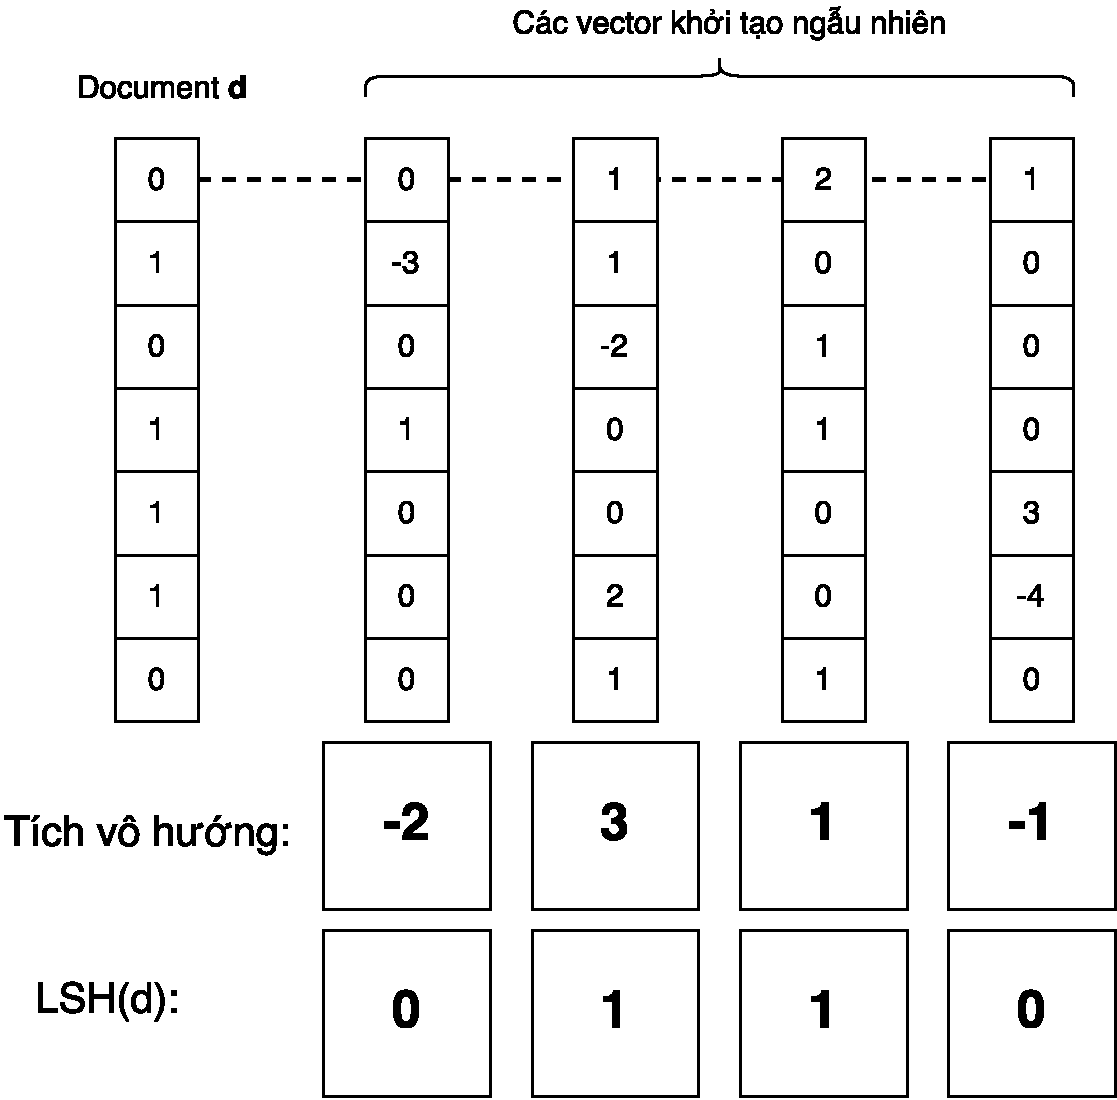
\includegraphics[width=0.65\textwidth]{LSH.pdf}
			\caption{Cách tính hash code cho một document trong một hash table}
		\end{center}
	\end{figure}
	
	\subsubsection{Mã giả}
	\begin{algorithm}[H]
		\caption{Phát hiện tin nóng sử dụng Locality Sensitive Hashing}
		\begin{algorithmic}[1]
			\REQUIRE luồng bài viết từ Twitter, giá trị ngưỡng t
			\ENSURE những cụm bài viết
			\State Khởi tạo L hash tables
			\ForEach{document $d$ mới}
				\ForEach{hash table $l$ trong $L$}
					\State Tính hash code cho document d: $LSH_l(d)$
					\State Thêm tất cả các documents d' có $LSH_l(d') = LSH_l(d)$ vào tập $S$
				\ENDFOR
				\State $dis_{min}(d) = 1$
				\ForEach{document $d'$ trong $S$}
					\IF {$distance(d,d') < dis_{min}(d)$}
					\STATE $dis_{min}(d) = distance(d,d')$
		 			\ENDIF
				\ENDFOR
				\IF{$dis_{min}(d) >= t$}
					\STATE tạo cụm mới chứa d
				\ELSE
					\STATE thêm d vào cụm chứa hàng xóm gần nhất của d
				\ENDIF
			\ENDFOR
			
		\end{algorithmic}
	\end{algorithm}
	Chú thích thuật toán:
	\begin{itemize}
		\item $t$: ngưỡng để xét một document có phải là first story hay không
		\item $LSH_l(d)$: hash code của document $d$ trong hash table thứ $l$
		\item $dis_{min}(d)$: khoảng cách giữa document $d$ với document gần nhất
		
	\end{itemize}
	
	Ưu điểm:
	\begin{itemize}
		\item Chi phí tính toán thấp do không cần so sánh toàn bộ các document với nhau.
		\item Độ chính xác tương đối tốt
	\end{itemize}

	Nhược điểm:
	\begin{itemize}
		\item Cần tìm chọn các thông số như: số lượng hash table, số lượng bit trong hash code,… tốt để cho kết quả chính xác.
		\item Có thể không tìm được document thật sự tương đồng nhất, trong trường hợp các điểm không được chia vào cùng vùng trong không gian do cách thiết lập của các siêu phẳng trong hash tables.
	\end{itemize}
	
	\subsubsection{LSH cải tiến}
	Dựa vào dữ liệu thực nghiệm của mình, Sasa Petrovic và cộng sự \cite{Petrovic:LSH} đưa ra nhận định rằng việc áp dụng LSH thuần túy vào bài toán FSD cho ra kết quả chưa tốt. Trong trường hợp điểm dữ liệu cách xa tất cả điểm còn lại, LSH không tìm được láng giềng gần nhất, do không có điểm nào khác rơi vào cùng bucket trong các hash table, dẫn đến không có điểm dữ liệu khác để so sánh. 
	
	Để giải quyết vấn đề này, Petrovic đưa ra phương án: mỗi khi tìm ra document $d$ có $dis_{min}(d)$ lớn hơn ngưỡng, ta áp dụng thuật toán tìm láng giềng gần nhất giữa document $d$ và khoảng 1000 tới 3000 document có thời gian gần đây nhất trong hệ thống, cập nhật giá trị $dis_{min}(d)$ và xét xem nó vẫn vượt ngưỡng hay không, nếu có thì ta kết luận $d$ là một first story, ngược lại ta cho $d$ vào cụm của láng giềng gần nó nhất.
	
	\begin{algorithm}[H]
		\caption{Phát hiện tin nóng sử dụng Locality Sensitive Hashing kết hợp với Nearest Neighbor Search}
		\begin{algorithmic}[1]
%			\boldmath
			\REQUIRE luồng bài viết từ Twitter, giá trị ngưỡng t
			\ENSURE những cum bài viết
			\State Khởi tạo L hash tables
			\ForEach{document $d$ mới}
				\ForEach{hash table $l$ trong $L$}
					\State Tính hash code cho document d: $LSH_l(d)$
					\State Thêm tất cả các documents d' có $LSH_l(d') = LSH_l(d)$ vào tập $S$
				\ENDFOR
				\State $dis_{min}(d) = 1$
				\ForEach{document $d'$ trong $S$}
					\unboldmath
					\IF {$distance(d,d') < dis_{min}(d)$}
					\State $dis_{min}(d) = distance(d,d')$
					\ENDIF
				\ENDFOR
				\IF{$dis_{min}(d) >= t$}
					\State Tính khoảng cách giữa d với một lượng (1000-3000) documents mới nhất trong bộ dữ liệu, cập nhật $dis_{min}(d)$ nếu có thay đổi.
				\ENDIF
				\IF{$dis_{min}(d) >= t$}
					\STATE tạo cụm mới chứa d
				\ELSE
					\STATE thêm d vào cụm chứa hàng xóm gần nhất của d
				\ENDIF
			\ENDFOR		
			
		\end{algorithmic}
	\end{algorithm}

\section{Giới thiệu một số độ đo đánh giá hiệu năng gom cụm} \label{clusterEvalMetrics}
Đánh giá chất lượng của kết quả gom cụm là nhiệm vụ khó khăn và phức tạp, do bản chất không hoàn toàn rõ ràng về định nghĩa của một "cụm". Theo tác giả Pang-Ning Tan và cộng sự \cite{IntroToDM}, có 3 loại phương pháp để đánh giá chất lượng cụm: 
	\begin{itemize}
		\item Đánh giá ngoại, có giám sát (External evaluation): Các độ đo có sử dụng thông tin bên ngoài như nhãn lớp của dữ liệu để so sánh với kết quả gom cụm.
		VD: Purity, Rand measure,…
		\item Đánh giá nội, không giám sát (Internal evaluation): Chỉ dựa vào các thông tin, thuộc tính có sẵn trong cụm để đánh giá.
		VD: Silhouette index, Dunn index, Davies–Bouldin index…
		\item Đánh giá tương đối (Relative evaluation): So sánh kết quả giữa các phương pháp gom cụm hoặc giữa các cụm, có thể dùng độ đo ngoại lẫn nội.
	\end{itemize}

%Khóa luận này chỉ xem xét đến các chỉ số đánh giá nội, do hạn chế về mặt dữ liệu tin tức có gán nhãn lớp.
	\subsection{Khoảng cách cục bộ và toàn cục (Intra-cluster và Inter-cluster distance)} \label{localglobaldistance}
	Hai độ đo này thuộc loại đánh giá nội, chỉ dựa vào chính dữ liệu được gom cụm để tính giá trị của chúng. Khoảng cách cục bộ của một cụm thể hiện mức độ các điểm dữ liệu trong một cụm tương đồng với nhau thế nào. Dưới đây là 3 cách để tính khoảng cách cục bộ:
		\begin{itemize}
			\item Dùng khoảng cách giữa 2 điểm xa nhau nhất trong cụm:\\
			\scalebox{1.1}{$intraclusterDistance(C_i) = \ max_{x, y \in C_i} distance(x, y)$}
			
			\item Dùng trung bình khoảng cách giữa tất cả cặp điểm trong cụm:\\
			\scalebox{1.1}{$intraclusterDistance(C_i) = \frac{1}{size(C_i) \ *\ [size(C_i)-1]} \sum_{x, y \in C_i, x \ne y} distance(x, y)$ }\\
			
			\item Dùng trung bình khoảng cách giữa từng điểm với tâm cụm:\\
			\scalebox{1.1}{$intraclusterDistance(C_i) = \frac{\sum_{x \in C_i} distance(x, \mu)}{size(C_i)} $, $\mu = \frac{\sum_{x \in C_i} x}{size(C_i)}$}\\	
		\end{itemize}
	
	Khoảng cách toàn cục là giá trị cho thấy mức độ rời rạc giữa tất cả các cụm với nhau, được tính bằng trung bình khoảng cách giữa các cụm:
		\begin{equation}
			interclusterDistance = \frac{1}{size(C) * [size(C)-1]} \sum_{C_i, C_j \in C} distance(C_i, C_j)
		\end{equation}
	
	Trong đó, khoảng cách giữa 2 cụm $distance(C_i, C_j)$ cũng có thế được xác định bằng nhiều cách như:
		\begin{itemize}
			\item Dùng khoảng cách giữa 2 điểm xa nhau nhất trong 2 cụm:\\
			\scalebox{1.1}{$distance(C_i, C_j) = \ max_{x \in C_i, y \in C_j} distance(x, y)$}
			
			\item Dùng trung bình khoảng cách giữa tất cả cặp điểm trong 2 cụm:\\
			\scalebox{1.1}{$distance(C_i, C_j) = \frac{1}{size(C_i) + size(C_j)} \sum_{x \in C_i, y \in C_j} distance(x, y)$ }
			
			\item Dùng khoảng cách giữa 2 tâm cụm:\\
			\scalebox{1.1}{$distance(C_i, C_j) = distance(\mu_{C_i}, \mu_{C_j})$, với $\mu_{C_i} = \frac{\sum_{x \in C_i} x}{size(C_i)}$}
%			\scalebox{1.1}{$\mu_{C_i} = \frac{\sum_{x \in C_i} distance(x, \mu)}{size(C_i)}$}\\	
	\end{itemize}

	Chú thích kí hiệu: 
	\begin{itemize}
		\item $C_i$: cụm dữ liệu thứ $i$
%		\item $localDistance(C_i)$: khoảng cách cục bộ của cụm $i$
		\item $x, y$: 2 điểm dữ liệu bất kì
		\item $distance(x, y)$: khoảng cách giữa 2 điểm dữ liệu, dùng các khoảng cách ở mục~\ref{distances}
		\item $size(C_i)$: số lượng điểm dữ liệu được gom vào cụm $i$
	\end{itemize}
	\subsection{Độ đo Dunn index}
	Dunn index được đề xuất bởi J. C. Dunn \cite{dunn1973fuzzy2}, độ đo này thể hiện mức độ gắn kết của từng cụm lẫn độ rời rạc giữa các cụm. Giá trị Dunn index được tính theo công thức sau:	
		\begin{equation} \label{dunnindex}
		DI = \frac{min_{1 \leq i \leq j \leq n}distance(C_i, C_j)}{max_{1 \leq k \leq n}intraclusterDistance(k)}
		\end{equation}
		
		Với $n$ là tổng số cụm thu được, và intraclusterDistance được tính theo một trong những cách ở mục~\ref{localglobaldistance}.
		
	Giá trị Dunn index càng cao thì các cụm càng tách biệt nhau và mỗi cụm thì có những điểm dữ liệu gom sát với nhau. Tuy vậy, mẫu số trong công thức (\ref{dunnindex}) lấy khoảng cách cục bộ của cụm rời rạc nhất chứ không lấy trung bình tất cả cụm, nên giá trị Dunn index là trường hợp xấu nhất chứ không phải trường hợp trung bình.
	\subsection{Hệ số Silhouette (Silhouette coefficient)}
%	Cohesion và separation
	
	Silhouette là một độ đo xem xét các đối tượng trong dữ liệu có được gán vào cụm hợp lý hay không, thông qua việc so sánh cả độ gắn kết của từng cụm và độ rời rạc giữa các cụm. Với mỗi điểm dữ liệu, giá trị silhouette coefficient nằm trong khoảng từ -1 đến 1, giá trị này cao khi điểm dữ liệu tương đồng với cụm của nó và ít tương đồng với cụm khác, và ngược lại. 
	
	Cách tính hệ số Silhouette cho một điểm dữ liệu \textbf{i} như sau:
	\begin{enumerate}
		\item Tính khoảng cách trung bình giữa i với các điểm trong cùng cụm với i. Gọi giá trị này là $a_i$.
		\item Với mỗi cụm g không chứa i, tính khoảng cách của i đến cụm g bằng trung bình khoảng cách giữa i với từng điểm trong cụm g, chọn cụm có khoảng cách đến i \textit{nhỏ nhất}. Gọi giá trị này là $b_i$
		\item Tính hệ số Silhouette theo công thức sau:
		\begin{equation}
		s(i) = \frac{b_i - a_i}{max\{a_i,b_i\}}
		\end{equation}
	\end{enumerate}
	
	Ở đây $a_i$ đại diện cho độ bất phù hợp của điểm i với cụm của nó, và $b_i$ đại diện cho độ tương đồng giữa điểm i với cụm gần nhất không chứa i. Vì vậy khi $a_i$ nhỏ, $b_i$ lớn, giá trị hệ số silhouette tiến tới 1, nghĩa là điểm dữ liệu i rất phù hợp với cụm của nó và không phù hợp với cụm khác. Trong trường hợp ngược lại, giá trị silhouette tiến tới -1.
	
	Giá trị hệ số Silhouette cho một kết quả phân cụm được tính bằng trung bình hệ số Silhouette của tất cả điểm dữ liệu.

	\subsection{Độ đo Purity}
	Đây là một độ đo đánh giá ngoại. Dựa trên nhãn lớp của dữ liệu, purity là độ đo về tính thuần khiết/độ đồng nhất của các cụm. Giá trị này tính bằng cách lấy tần số của lớp chiếm số lượng nhiều nhất trong cụm (tính theo phần trăm kích cỡ cụm). Purity càng cao khi cụm chứa càng nhiều điểm dữ liệu thuộc cùng một nhãn lớp.\\
	
	Giá trị purity của một cụm $C_i$ được tính bằng công thức:
	\begin{equation}
	purity(C_i) = max_j( \frac{m_{ij}}{m_i})
	\end{equation}
	
	Trong đó:
	\begin{itemize}
		\item $m_i$: số điểm dữ liệu thuộc cụm i
		\item $m_{ij}$: số điểm dữ liệu thuộc lớp j và nằm trong cụm i
	\end{itemize}
	
	Giá trị purity của tất cả cụm được tính như sau:
	\begin{equation}
	purity = \sum_{i=1}^{K} \frac{m_i}{m} \ purity(C_i)
	\end{equation}
	
	Trong đó:
	\begin{itemize}
		\item $K$: tổng số cụm
		\item $m$: tổng số điểm dữ liệu
	\end{itemize}
	
\section{Xếp hạng cụm}
	Một yêu cầu của bài toán phát hiện tin nóng là các chuỗi tin (ứng với các cụm) phải được sắp xếp theo mức độ nóng giảm dần. Hầu hết các phương pháp đã khảo sát trong khóa luận này chỉ tập trung vào việc gom cụm và cải thiện chất lượng cụm, mà không đề cập đến việc sắp xếp cụm theo thứ tự nào đó. 
	
	Tác giả Phuvipadawat đưa ra một số công thức để tính điểm lượng giá độ nóng của chuỗi tin, và các chuỗi tin được sắp xếp theo giá trị điểm giảm dần \cite{SwitPhuvipadawat}.
	
%	Các cụm được xếp hạng bằng công thức được đề xuất bởi Phuvipadawat \cite{SwitPhuvipadawat}, mỗi cụm được gán một giá trị điểm, và dùng điểm đó để so sánh giữa các cụm, cụm có điểm cao nhất sẽ được sắp xếp lên đầu.
	
	Điểm này cân nhắc tầm ảnh hưởng của những người viết bài trong cụm, cũng như mức độ lan tỏa của chính các bài viết trong cụm. Giá trị điểm cũng được cập nhật thường xuyên và sẽ giảm dần theo thời gian nếu không có những bài viết mới làm tăng điểm cho nó. So với công thức của Phuvipadawat, công thức 2.12 bổ sung thêm yếu tố lượng favorite của cụm, do đây cũng là một thành phần ghi nhận phản ứng từ người dùng Twitter.
	
	Giá trị điểm xếp hạng của một cụm $C_i$ được cho bằng công thức sau:
	\begin{equation}
		Score(C_i) = \frac{1}{Z} \sum_{j = 1}^k \frac{S_i}{log_2(\Delta_j + 2)}
	\end{equation}
	
	Với $S_i$ tính bằng:
	\begin{multline}
	S_i = w_1 \sum_{u_i \in C_i} FollowerCount(u_i) + w_2\ TotalRetweetCount(C_i)\\ + w_3\ TotalFavoriteCount(C_i)
	\end{multline}

	Trong đó:
	\begin{itemize}
		\item $\frac{1}{Z}$: giá trị để chuẩn hóa điểm cụm, Z là tổng điểm của các cụm khi chưa chuẩn hóa
		\item $k$: số lượng document trong cụm
		\item $\Delta_j$: chênh lệch thời gian giữa thời điểm hiện tại với thời gian bài viết $j$ được đăng
		\item $w_1, w_2$: trọng số cho hai vế của biểu thức
		\item $u_i$: người dùng thứ $i$
		\item $FollowerCount(u_i)$: số người follow người dùng $u_i$ trên Twitter
		\item $TotalRetweetCount(g_i)$: tổng số retweet của các bài đăng trong cụm $c_i$
	\end{itemize}
\section{Kết chương}
Chương này đã phát biểu bài toán phát hiện tin nóng và đưa ra 4 thuật toán tiếp cận theo hướng gom cụm. Đồng thời trình bày về các độ đo tương đồng, độ đo đánh giá chất lượng cụm và cách xếp hạng cụm. Chương tiếp theo sẽ trình bày về việc xây dựng hệ thống phát hiện tin nóng.